\documentclass{article} % For LaTeX2e
\usepackage{nips15submit_e,times}
\usepackage{hyperref}
\usepackage{url}
\usepackage{multirow}
\usepackage{array}
\usepackage{amsmath}
\usepackage{graphicx}
\graphicspath{ {./} }
\newcolumntype{M}[1]{>{\centering\arraybackslash}m{#1}}
%\documentstyle[nips14submit_09,times,art10]{article} % For LaTeX 2.09


\title{CHORDR: Hidden-Markov-Perceptron for Chord Recognition}


\author{
David S.~Hippocampus\thanks{ Use footnote for providing further information
about author (webpage, alternative address)---\emph{not} for acknowledging
funding agencies.} \\
Department of Computer Science\\
Cranberry-Lemon University\\
Pittsburgh, PA 15213 \\
\texttt{hippo@cs.cranberry-lemon.edu} \\
\And
Coauthor \\
Affiliation \\
Address \\
\texttt{email} \\
\AND
Coauthor \\
Affiliation \\
Address \\
\texttt{email} \\
\And
Coauthor \\
Affiliation \\
Address \\
\texttt{email} \\
\And
Coauthor \\
Affiliation \\
Address \\
\texttt{email} \\
(if needed)\\
}

% The \author macro works with any number of authors. There are two commands
% used to separate the names and addresses of multiple authors: \And and \AND.
%
% Using \And between authors leaves it to \LaTeX{} to determine where to break
% the lines. Using \AND forces a linebreak at that point. So, if \LaTeX{}
% puts 3 of 4 authors names on the first line, and the last on the second
% line, try using \AND instead of \And before the third author name.

\newcommand{\fix}{\marginpar{FIX}}
\newcommand{\new}{\marginpar{NEW}}

%\nipsfinalcopy % Uncomment for camera-ready version

\begin{document}


\maketitle

\begin{abstract}
Analysis of harmonic structure in music often starts with labelling every chord in a musical piece. A system for performing chord recognition is very useful for harmonic analysis and for applications such as music search, music similarity identification and music composition. In this report, we present CHORDR, an improved model for automatic chord recognition based on BREVE’s HMPerceptron model \cite{breve}. We compare our results validated on a corpus of chorales from JS Bach and various other classical compositions.
\end{abstract}

\section{Introduction}

Our system takes a MIDI input re-encoded as a list of events. Each event contains information of the frequency of the twelve pitch classes played, the bass note, and its meter (relative accent). We aim to assign each event a chord label - a set of simultaneously played notes.

We also take into consideration chord progressions and accents as contextual information. We consider an event as “vertical” information and the events that occur around it as “horizontal” information. Together, they form the framework for evaluating our features functions.

We approach the chord recognition problem as a sequential supervised learning (SSL) problem. For each training piece $m$, we denote the form $(X_m, Y_m)$, where $X_m = (x_{m,1},\ldots,x_{m,Tm})$ is a sequence of $T_m$ events and $Y_m = (y_{m,1},\ldots,y_{m,Tm})$, are the corresponding chord labels. Using the HMPerceptron model, we obtain a classifier H that given a new sequence of pieces $X$, predicts the corresponding chord labels $Y=H(X)$ as follows \cite{breve}:

\begin{equation}
  H(X) = \arg\max_{Y'={y'_1\ldots y'_T}}\sum_t^{}\sum_s^{}\mathbf{w}_s\phi_s(X,y'_t,y'_{t-1})
\end{equation}

where $\phi_s$ are boolean feature functions of the sequence of events X and the previous and current labels.

Finding the classifier H is essentially a path-finding problem over a layered-graph. Here, the vertices represent chord labels which are weighted using vertical basis functions, while transitional weights are calculated using horizontal basis functions. With $T$ layers, and $K$ labels, we have a $T \times K$ graph. Finding the optimal path can be solved using Viterbi algorithm, yielding a complexity of $\Theta(TK^2)$. However, our system uses CarpeDiem algorithm, solving the problem in $\Theta(TKlog(k))$.

\section{Model Formulation}

BREVE’s CarpeDiem path-finding algorithm \cite{carpediem} is already highly efficient and we don’t think it needs further improvement. However, we found the original 43 feature functions lacking in functionality. We first describe the problems of BREVE’s feature functions and then present our improvements through CHORDR’s feature functions. We denote the current event with $x_t$, and the currently predicted label with $y_t$.

\subsection{A critique of BREVE's Feature Functions}

In BREVE, five consecutive entries in the feature vector are used to indicate exactly how many notes of $y_t$ are present in $x_t$. Unfortunately, some chord structures contain 3 distinct notes, while others, like the dominant seventh chord, contain 4 distinct notes. Of the supported chord types, approximately half of the chord structures are comprised of 4 distinct notes, however, these chords are used less frequently. As a result, the learned weights prioritize having three notes of $y_t$ present in $x_t$, which diminishes the discriminative power of this feature. Consider an event $x_t$, which contains the pitch classes $C$, $E$, $G$, and $B\flat$. Here, $x_t$ is a fully stated dominant seventh chord, yet it contains 3 distinct notes of $A_{m7}$, $E_{m6}$, $C_{M}$, $C_{M4}$, $C_{M6}$, $C_{M7}$, $G_{d}$, while containing 4 distinct notes of $C_V$. In general this feature aims to gauge the similarity between a collection of notes and a chord label, however this approach is not optimal, as it reports $C_V$ to be less likely than a number of other labels.

Alternatively, CHORDR uses five consecutive entries in the feature vector to indicate the percentage of notes in $x_t$ which are contained in $y_t$. Notably, the percentage is quantized into partitions each with a width of $20\%$. Using this approach, the learnt weights reflect the fact that having $(80\% - 100\%]$ is the most desirable condition for a predicted label. As a result, both the training error and the testing error decreased using this metric.

Furthermore, the model adopted in BREVE makes the assumption that the presence of each note within a given chord structure is equally significant, when in fact this is not the case. For example, given a $C_{M7}$ chord, or any seventh chord for that matter, the presence or absence of a fifth is a very weak indicator, as it is quite common to voice seventh chords without the fifth. In contrast, the presence or absence of a seventh is extremely important, as this chord type specifically dictates its presence. With this in mind, it is somewhat surprising that Radicioni et al. have two features which indicate if the root and added note of a chord $y_t$ are present in $x_t$, but neglect to observe the presence of a third or fifth. Additionally, it seems counterintuitive that BREVE only observes if the root of yt is present in $x_{t+1}$, neglecting to consider the content of $x_{t-1}$. In light of this reality, CHORDR reports the presence of a third and fifth.

The most prominent difficulty in discerning the correct chord label is in cases where xt is contains a small number of distinct pitches. Without contextual information, it is reasonable to assert that an event containing the pitch classes C and G may represent a $C_{m}$, $C_{M}$, $G_{M4}$ or $A\flat_{M7}$ chord. Quite frequently, a fully voiced chord is not sounded simultaneously, as the remaining chord tones have been stated previously or are to be stated on the following beat. In order to mitigate these uncertain circumstances, contextual analysis is necessary.

\subsection{Determining the Relevance of CHORDR}

Unfortunately, it is not admissible to take adjacent events into consideration for every input $x_t$, as the nature of adjacent events is only illuminating in specific circumstances. Upon experimenting with several methods for determining a relevant set of events, the joint criterion of event similarity and accent trajectory was determined to be sufficient.

In order to evaluate the similarity between two events $x_A$ and $x_B$, the number of common tones, or equivalently the number of elements in $x_A \cap x_B$, are counted. When this value surpasses a threshold, the events are considered to be similar. In most musical genres, chord changes are accented. As a result, a set of unaccented events following an accented event frequently constitutes a single chord structure. Since accents are relative to the surrounding context, a pair of events $x_A$ and $x_A+1$ satisfy the accent condition when $x_A$ is less accented than $x_{A+1}$. With regards to the music of J.S. Bach and his Baroque contemporaries, accented beats are directly derived from the metric structure. Accordingly, chord changes often occur on strong beats. Although this musical convention has decreased in prevalence since the Baroque era, chord changes are consistently accented despite the fact that these accents may be syncopated. Additionally, MIDI files contain velocity information which may be used to extrapolate the required accent information. Consequently, this analysis is not limited to the music of J.S. Bach, as it is dependent on accent trajectory not metric structure.

Let $x_R$ be a set of consecutive events, necessarily including $x_t$, which collectively satisfy the similarity condition and accent condition. Then, $x_R$ is constructed as follows. To begin, $x_t$ is the only element contained in $x_R$. Here, $x_t.\text{accent}$ refers to the relative accent of event $t$, an integer in [1, 5]. Given $L < t$, and $x_{L+1} \in xR$, $x_L$ satisfies the accent condition if $x_L.\text{accent} > x_{L+1}.\text{accent}$ and the similarity condition if $|x_L \cap x_t| > \text{threshold}$. Given $L > t$, and $x_L-1 \in x_R$, $x_L$ satisfies the accent condition if $x_L.\text{accent} < x_{L-1}.\text{accent}$ and the similarity condition if $|x_L \cap x_t| > \text{threshold}$. To reiterate, $x_L$ is an eligible addition to $x_R$ if it directly precedes or follows one of the events in $x_R$ and satisfies the similarity condition and the accent condition.

\begin{tabular}{ r | c c c c c c c }
  \textbf{Events}        & $x_{28}$ & $x_{29}$ & $x_{30}$ & $x_{31}$ & $x_{32}$ & $x_{33}$ & $x_{34}$ \\
  \textbf{Label}         & $D_{m7}$ & $D_{m7}$ & $D_{m7}$ & $G_M$ & $C_M$ & $F_M$ & $F_M$ \\
  \textbf{Metric Accent} & 5 & 2 & 1 & 3 & 4 & 3 & 2 \\
\end{tabular}

For added clarity, an excerpt from the J.S. Bach dataset will be analyzed, as shown in Table 1. Without considering similarity, $x_R = \{ x_{28}, x_{29}, x_{30} \}$ with $28 \leq t \leq 30, x_R = \{ x_{31} \}$ with $t = 31$, and $x_R = \{ x_{32}, x_{33}, x_{34} \}$ with $32 \leq t \leq 34$. Evidenced by the correct chord labels provided above, this segmentation of events is quite reasonable, however, it is evident that the similarity condition is needed to disassociate $x_{32}$ from $\{ x_{33}, x_{34} \}$.

\subsection{An Overview of Feature Functions in CHORDR}

Upon determining $x_R$, several feature functions make observations on general subsets of $x_R$. Notably, in some cases these subsets may be completely empty, and in that case such features report 0. Let $x_C$ be the set difference of $x_R - x_t$, such that $x_C$ contains all contextually relevant events with the exclusion of $x_t$. Let $x_S$ be the set intersection of all events in $x_R$, such that $x_S$ only contains pitch classes common to all contextually relevant events.

Here, one will briefly rationalize the importance each aforementioned subset of $x_R$. Clearly, it is important to exclusively consider the contents of xt as it is the event we are interested in labelling. Similarly, it is essential to consider the nature of $x_C$, in accordance with the reasons for contextual analysis discussed above. With regards to $x_S$, quite frequently this set contains very few pitch-classes, however, the presence of even a single pitch class in $x_S$, is significant. Often this pitch class is the root or the fifth of the correct chord label. As a result, it was not beneficial to report if $x_S$ is completely stated, as this case is extremely rare and would likely only occur with $x_R$ = $x_t$ = $x_S$. However, in that case this attribute is already captured by reporting if $x_t$ is completely stated.

Notably, accuracy was slightly improved when reporting the asserted-degree of $y_t$ on pitch classes shared by $x_t$ and $x_{t-1}$ or $x_{t+1}$ dependent on $x_R$ membership, in contrast to reporting the asserted-degree of yt with respect to each event in $x_R$. This is likely due to the fact that outermost events in $x_R$ are more likely to contain notes related to a previous chord structure (i.e suspensions) when $x_R$ contains more than 3 events. Since these features are dependent on the presence or absence of a single pitch class, they are quite sensitive to these unrelated pitches. Consequently, it is still relevant to consider $( x_R \cap y_t ) / |x_R|$ as the effects of these suspended pitches are significantly lessened. As an added measure, it was found beneficial to record the likelihood of a particular chord type, reported in features $[43, 43 + K - 1]$, where $K$ is number of label types. In the table below, the vertical feature functions are summarized, where highlighted rows signify feature functions developed independently for CHORDR. Notably, the horizontal features in BREVE were not modified.

\begin{table}
  \begin{tabular}{|M{4.5cm}|M{2cm}|M{6cm}|}

    \hline

    \textbf{$\mathbf{\phi}$ class} & \textbf{$\mathbf{\phi}$ number} & \textbf{$\mathbf{\phi}$ description} \\

    \hline

    Penalize Added Note on Weak Beats
    & $1$ & if $X.meter(t) < X.meter(t-1)$ and $y_t$ is an added note chord type $F(1) = 0$ \\

    \hline

    \multirow{4}{*}{Asserted-notes}
    & 2 & root of $y_t$ in $x_t$\\ \cline{2-3}
    & 3 & third of $y_t$ in $x_t$ \\ \cline{2-3}
    & 4 & fifth of $y_t$ in $x_t$ \\ \cline{2-3}
    & 5 & added note of $y_t$ in $x_t$ \\

    \hline

    \multirow{6}{*}{\parbox{4.5cm}{\centering Contextually Relevant Asserted-notes for each Chord Degree \{ root, third, fifth, added note \}}}
    & 6 & root of $y_t$ in $x_t \cap x_{t - 1} given x_{t - 1} in x_{R}$ \\ \cline{2-3}
    & $\dots$ & $\ldots$ \\ \cline{2-3}
    & 10 & root of $y_t$ in $x_t \cap x_{t + 1} given x_{t + 1} in x_{R}$ \\ \cline{2-3}
    & $\ldots$ & $\ldots$ \\ \cline{2-3}
    & 14 & root of $y_t$ in $x_s$ \\ \cline{2-3}
    & $\ldots$ & $\ldots$ \\

    \hline

    \multirow{2}{*}{\parbox{4.5cm}{\centering Root in Context Regardless of Relevance}}
    & 18 & root of $y_t$ in $x_{t - 1}$ \\ \cline{2-3}
    & 19 & root of $y_t$ in $x_{t - 1}$ \\

    \hline

    \multirow{3}{*}{\parbox{4.5cm}{\centering Completely Stated Chords}}
    & 20 & all notes of $y_t$ are in $x_t$ \\ \cline{2-3}
    & 21 & all notes of $y_t$ are in $x_t$ \\ \cline{2-3}
    & 22 & all notes of $y_t$ are in $x_t$ \\ \cline{2-3}

    \hline

    \multirow{4}{*}{\parbox{4.5cm}{\centering Percentage of Notes in $Y_t$ (For every 20\%)}}
    & 23 & $\frac{(x_t \cap y_t)}{|x_t|}$ \\ \cline{2-3}
    & $\ldots$ & $\ldots$ \\ \cline{2-3}
    & 28 & $\frac{(x_R \cap y_t)}{|x_R|}$ \\ \cline{2-3}
    & $\ldots$ & $\ldots$ \\ \cline{2-3}
    & 33 & $\frac{(x_C \cap y_t)}{|x_C|}$ \\ \cline{2-3}
    & $\ldots$ & $\ldots$ \\ \cline{2-3}
    & 38 & $\frac{(x_S \cap y_t)}{|x_S|}$ \\ \cline{2-3}

    \hline

    \multirow{3}{*}{\parbox{4.5cm}{\centering Chord Type Likelihood (K label types)}}
    & 43 & $y_t$ is chord type $M$ \\ \cline{2-3}
    & 44 & $y_t$ is chord type $M4$ \\ \cline{2-3}
    & $\ldots$ & $\ldots$ \\

    \hline

    \multirow{8}{*}{\parbox{4.5cm}{\centering Bass-at-degree}}
    & 43 + K & root of $y_t$ is bass note of $x_t$ \\ \cline{2-3}
    & 44 + K & third of $y_t$ is bass note of $x_t$ \\ \cline{2-3}
    & 45 + K & fifth of $y_t$ is bass note of $x_t$ \\ \cline{2-3}
    & 46 + K & seventh of $y_t$ is bass note of $x_t$ \\ \cline{2-3}
    & 47 + K & root of $y_t$ is bass note of $x_{t+1}$ \\ \cline{2-3}
    & 48 + K & fifth of $y_t$ is bass note of $x_{t+1}$ \\ \cline{2-3}
    & 49 + K & root of $y_t$ is bass note of $x_{t+1}$ \\ \cline{2-3}
    & 50 + K & fifth of $y_t$ is bass note of $x_{t+1}$ \\

    \hline

  \end{tabular}
\end{table}


\begin{table}
  \begin{tabular}{|M{3.5cm}|M{0.25cm}|M{3.5cm}|M{3cm}|M{1cm}|M{3cm}|}
    \hline

    \textbf{$\phi$ class} & & \textbf{$\phi$ description} & \textbf{$\phi$ class} & & \textbf{$\phi$ description} \\

    \hline

    % Row 1

    Penalize Added Note on Weak Beats

    & 1 & if X.meter(t) < X.meter(t-1) and yt is an added note chord type F(1) = 0 &

    \multirow{4}{*}{\parbox{3cm}{\centering Percentage of Notes in Yt (For every 20\%)}}

    & 23 & $( x_t \cap y_t ) / |x_t|$ \\ \cline{1-3}\cline{5-6}

    % Row 2

    \multirow{4}{*}{\parbox{3.5cm}{\centering Asserted-notes}}

    & 2 & root of $y_t$ in $x_t$ &
    & 28 & $( x_R \cap y_t ) / |x_R|$ \\ \cline{2-3}\cline{5-6}

    % Row 3

    & 3 & third of $y_t$ in $x_t$ &
    & 33 & $( x_C \cap y_t ) / |x_C|$ \\ \cline{2-3}\cline{5-6}

    % Row 4

    & 4 & fifth of $y_t$ in $x_t$ &
    & 38 & $( x_S \cap y_t ) / |x_S|$ \\ \cline{2-6}

    % Row 5

    & 5 & added note of $y_t$ in $x_t$ &

    \multirow{3}{*}{\parbox{3cm}{\centering Chord Type Likelihood (K label types)}}

    & 43 & $y_t$ is chord type $M$ \\ \cline{1-3}\cline{5-6}

    % Row 6

    \multirow{6}{*}{\parbox{3.5cm}{\centering Contextually Relevant Asserted-notes for each Chord Degree \{ root, third, fifth, added note \}}}

    & 6 & root of $y_t$ in $x_t$ ∩ $x_{t-1}$ given $x_{t-1}$ in $x_R$ &
    & 44 & $y_t$ is chord type $M4$ \\ \cline{2-3}\cline{5-6}

    % Row 7

    & $\ldots$ & $\ldots$ &
    & $\ldots$ & $\ldots$ \\ \cline{2-6}

    % Row 8

    & 10 & root of $y_t$ in $x_t \cap x_{t+1}$ given $x_{t+1}$ in $x_R$ &

    \multirow{8}{*}{\parbox{3cm}{\centering Bass-at-degree}}

    & $43 + K$ & root of $y_t$ is bass note of $x_t$ \\ \cline{2-3}\cline{5-6}

    % Row 9

    & $\ldots$ & $\ldots$ &
    & $44 + K$ & third of $y_t$ is bass note of $x_t$ \\ \cline{2-3}\cline{5-6}

    % Row 10

    & 14 & root of $y_t$ in $x_S$ &
    & $45 + K$ & fifth of $y_t$ is bass note of $x_t$ \\ \cline{2-3}\cline{5-6}

    % Row 11

    & $\ldots$ & $\ldots$ &
    & $46 + K$ &  seventh of $yt$ is bass note of xt \\ \cline{1-3}\cline{5-6}

    % Row 12

    \multirow{2}{*}{\parbox{3.5cm}{\centering Root in Context Regardless of Relevance}}

    & 18 & root of $y_t$ in $x_{t-1}$  &
    & $47 + K$ & root of $y_t$ is bass note of $x_{t+1}$ \\ \cline{2-3}\cline{5-6}

    % Row 13

    & 19 & fifth of $y_t$ is bass note of $x_{t+1}$  &
    & $48 + K$ & fifth of $y_t$ is bass note of $x_{t+1}$ \\ \cline{1-3}\cline{5-6}

    % Row 14

    \multirow{3}{*}{\parbox{3.5cm}{\centering Completely Stated Chords}}

    & 20 & all notes in $y_t$ are in $x_t$ &
    & $49 + K$ & root of $y_t$ in $x_{t}$ \\ \cline{2-3}\cline{5-6}

    % Row 15

    & 21 & all notes in $y_t$ are in $x_R$ &
    & $50 + K$ & \\ \cline{2-6}

    % Row 16

    & 22 & all notes in $y_t$ are in $x_S$ &
    & $51 + K$ &  \\ \cline{2-3}\cline{5-6}

    \hline

  \end{tabular}
\end{table}

\section{Experiments}

\subsection{Datasets}

We evaluated our chord recognition algorithm and compared the results using BREVE and CHORDR basis functions on two datasets: the JS Bach Chorales \cite{coral}, and a subset of pieces from the Kostka-Payne (KP) corpus \cite{kpcorpus}. JSBach contained 60 pieces of the same musical style and composer, totalling 5665 events. KP contained 29 pieces of various classical composers with differences in style, totalling 2273 events. Both datasets contained 108 unique chord labels, however, not all the same. The union of both chord label sets totalled 132 unique chord labels.

We constructed the KP dataset by using a MIDI to CSV extraction tool \cite{midicsv} to obtain the pitch classes and chord labels (annotated by an expert) from the MIDI files. The meter attributes were obtained using Melisma’s meter analyzer \cite{mitpress}. The results were then formatted to be consistent with the JSBach dataset.

\subsection{Test}

In a simplified model, we first tried classifying the chords with respect to their primary mode $(M, m, d)$, ignoring all added notes. This yielded 36 classification labels, which was a good candidate for evaluating basic performance of the algorithm. We then extended our tests to classify the full chord labels.

JSBach and KP were classified using their respective 108 chord labels. A combined test was also conducted on a fixed random permutation of the combined datasets using all 132 chord labels. All tests were conducted using 6 fold cross validation. Our results are summarized in figure E2.

\begin{table}
  \begin{tabular}{M{1.5cm} | M{3.5cm} M{3cm} | M{3.5cm} M{3cm}}
    \hline
    & \multicolumn{1}{l}{BREVE Basis Functions} & & \multicolumn{1}{l}{CHORDR Basis Functions} \\
    \hline
    Dataset (\# Pieces) & Simplified chord classification (M m d) & Full chord classification & Simplified chord classification (M m d) & Full chord classification \\

    \hline

    JSBach (60) & 73.85 & 64.46 & 84.22 & 78.56 \\

    \hline
    KP (29)  & 55.02 & 46.71 & 67.82 & 58.48 \\

    \hline
    Combined (89) & 74.45 & 59.76 & 82.09 & 69.39 \\

    \hline
  \end{tabular}
\end{table}

\section{Error Analysis}

Chord recognition performed much better on the JSBach dataset compared to the KP dataset because the contents of KP contained a higher variance of chord patterns. We thought it was interesting nonetheless to experiment with a different dataset to gauge how chord recognition performed in a broader context. Classification on the combined dataset performed somewhere in between JSBach and KP. There was also a higher variance in each fold validation due to a larger set of labels being classified.

\subsection{Misclassifications - BREVE vs. CHORDR}

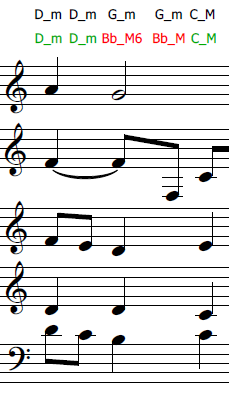
\includegraphics[scale=0.5]{relative_error.PNG}
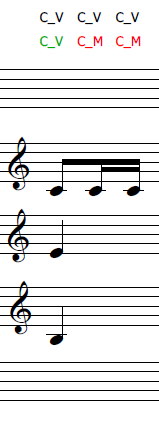
\includegraphics[scale=0.5]{VM_error.PNG}
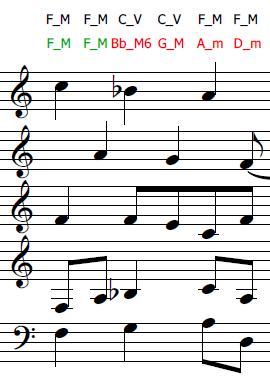
\includegraphics[scale=0.5]{other_error.PNG}

For the full chord classification on the JSBach dataset, around 36\% of chords were misclassified using BREVE compared to 21\% using CHORDR. Furthermore, there are two major classes of misclassified chords: relative key errors (24\% of the error), and added note misclassifications (28\% of the error).

Relative key errors occur due to the duality of relative major and minor keys in musical theory. From a learning perspective, relative chords tend to overlap in notes, making it difficult for the classifier to distinguish. In our experiments, CHORDR reduced this type of error by 25\% compared to BREVE. (SEE FIGURE ANALYSIS-TOPLEFT)

Added note misclassifications occur when a classified chord is off by a single added note. The majority of these cases are dominant 7th chords being mistaken for major chords. This is common because not only there is a one note difference in the added note of the chord between a V and a M chord, but both chords sound nearly identical from a musical perspective. Contextual information is absolutely necessary to classify these, but is often not enough, due to the interchangeability between these two chords. In our experiments, CHORDR reduced this type of error by 38\% compared to BREVE. (SEE FIGURE ANALYSIS-TOPMID)

The majority of the remaining error cases were of chords mixed with passing tones identified as an inversion of a completely different chord. These errors are non trivial to resolve. Sometimes the problem is due to chord changes on unusual beats or strange rhythms of the chord progression. Other times, there is not enough specific occurrences of the chord progressions for the algorithm to learn on. The HM model is at a disadvantage here because the influence of the basis functions that govern the classification of these special cases are undermined by the more common basis functions. (SEE FIGURE ANALYSIS-TOPRIGHT)

(Image goes here)

Figure (ANALYSIS): Visualization of some misclassifications on 000106b\_ of JSBach. Green indicates a correct classification and red indicates a misclassification. (TOPLEFT) shows a misclassification due to relative key. (TOPMID) shows a misclassification due to incorrect added note. (TOPRIGHT) shows a misclassification due to unusual rhythm and chord changes on unaccented beats.

\section{Conclusion}

Based on our experiments, CHORDR is an improvement in chord recognition, increasing the classification accuracy from 65\% to 79\% when compared to our implementation of BREVE on the JS Bach dataset. This was an average increase in accuracy of 17\% across all datasets we tested on. In general, this discriminative hidden markov model allows more flexibility in the design of its feature functions through the incorporation of musical analysis. On the other hand, the hidden markov model is limited to information between adjacent layers, therefore losing some of the knowledge involved in complex chord progressions. Any further improvement to the accuracy would likely require to take into account more layers via higher order markov models or bayesian networks.

\begin{thebibliography}{9}

% 5 from google doc
\bibitem{breve}
  D. Radicioni and R. Esposito,
  \emph{BREVE: An HMPerceptron-Based Chord Recognition System},
  Advances In Music Retrieval,
  2010.

% 6 from google doc

\bibitem{carpediem}
  D. Radicioni and R. Esposito,
  \emph{CarpeDiem: Optimizing the Viterbi Algorithm and Application to Supervised Sequential Learning}
  Journal of Machine Learning Research,
  2009

% 1 from google doc
\bibitem{coral}
  D. Radicioni and R. Esposito,
  \emph{UCI Machine Learning Repository: Bach Choral Harmony Data Set},
  Archive.ics.uci.edu,
  [Online]. Available: https://archive.ics.uci.edu/ml/datasets/Bach+Choral+Harmony. [Accessed 10-Dec-2015]
  2014.

% 2 from google doc

\bibitem{kpcorpus}
  P. Bryan,
  \emph{KPCorpus},
  Cs.northwestern.edu. [Online]. Available: http://www.cs.northwestern.edu/~pardo/kpcorpus.htm. [Accessed: 10- Dec- 2015].

% 3 from google doc

\bibitem{midicsv}
  J. Walker,
  \emph{MIDICSV: Convert MIDI File to and from CSV},
  Fourmilab.ch. [Online]. Available: http://www.fourmilab.ch/webtools/midicsv/. [Accessed: 10- Dec- 2015],
  2015

% 4 from google doc
\bibitem{mitpress}
  D, Temperley,
  The Cognition of Basic Musical Structures,
  MIT Press, Cambridge, MASS,
  2014.

\end{thebibliography}

\end{document}
